\documentclass{beamer}
\usepackage{xcolor}
\usepackage{graphicx}
\usepackage{tikz}
\usepackage{multirow}
\usepackage{animate}

\usetikzlibrary{positioning}
\usetikzlibrary{shapes,arrows,positioning,shadows}

\definecolor{myblue}{RGB}{0, 120,204}
\definecolor{mygreen}{RGB}{0, 153, 0}

\usetheme{Madrid}

\setbeamertemplate{navigation symbols}{}
\setbeamercolor{structure}{fg=myblue}
\setbeamercolor{alerted text}{fg=red}

\title{\textbf{B+ Tree}}
\author[Anup \and  Afzal \and Asif]{\textbf{Anup Halder Joy - 2005005\\Afzal Hossan - 2005021\\Asif Karim - 2005024} }
\date{\today}
\setbeamerfont{title}{size=\huge}

\begin{document}

\frame{\titlepage}
\begin{frame}{Agenda}
  \tableofcontents
\end{frame}
\begin{frame}{}
    \begin{figure}
        \centering
        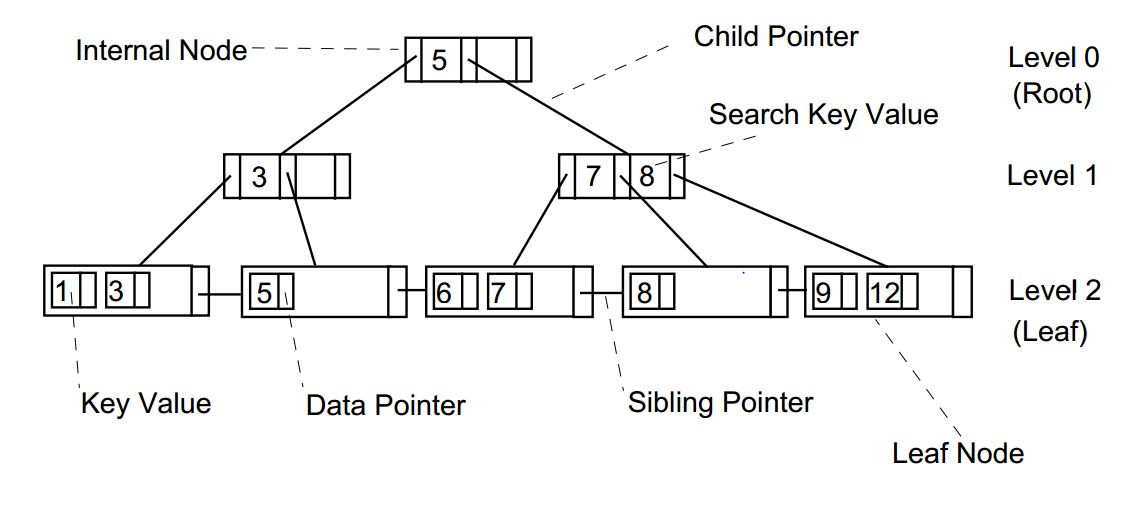
\includegraphics[scale=0.4]{Images/B+tree.jpg}
        \caption{B+ Tree}
    \end{figure}
\end{frame}

\begin{frame}{B+ Tree}
    \centering
    {\huge\alert{WHAT} is a B+ Tree?}
\end{frame}

\section{Introduction}

\begin{frame}{What is a B+ Tree?}
    \begin{block}{Definition of B+ Tree} 
        A B+ tree is an m-ary tree with a variable but often large number of children per node. A B+ tree consists of a root, internal nodes and leaves. \cite{navathe2010fundamentals}.
    \end{block}
    \begin{block}{}
         A \alert{B+ Tree} is a self-balancing tree data structure that maintains sorted data and allows searches, sequential access, insertions, and deletions
    \end{block}
\end{frame}

\section{History}

\begin{frame}{Inventors}
\begin{table}[]
    \centering
    \begin{tabular}{c c}
        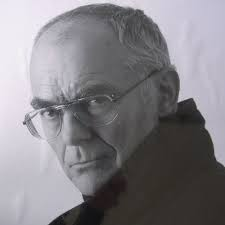
\includegraphics[scale = 0.5]{Images/Bayer.jpg} & 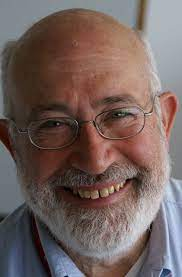
\includegraphics[scale = 0.5]{Images/Edward.jpg} \\
       \textit{Rudolf Bayer} & \textit{Edward M. McCreight} \\
    \end{tabular}
\end{table}    
\end{frame}

\begin{frame}{Evolution of B+ Tree}
    \tikzstyle{block} = [rectangle, draw, top color=blue!30, bottom color=blue!5, text width=8em, text centered, rounded corners, minimum height=3em]
    \tikzstyle{line} = [draw, -latex'] 

    \begin{table}[]
        \centering
        \begin{tabular}{c c}
            \begin{tikzpicture}[node distance=2cm, every node/.style={drop shadow}]
                % Nodes
                \onslide<1->{\node [block, fill=yellow] (bst) {Binary Search Tree};}
                \onslide<2->{\node [block, below of=bst, fill=yellow] (mWaytree) {M-way Tree};}
                \onslide<3->{\node [block, below of=mWaytree, fill=yellow] (btree) {B Tree};}
                \onslide<4->{\node [block, below of=btree, fill=yellow] (bplustree) {B+ Tree};}
            
                % Arrows
                \onslide<2->{\path [line] (bst) -- (mWaytree);}
                \onslide<3->{\path [line] (mWaytree) -- (btree);}
                \onslide<4->{\path [line] (btree) -- (bplustree);}
            \end{tikzpicture}
            &
            \begin{overprint}
                \onslide<1>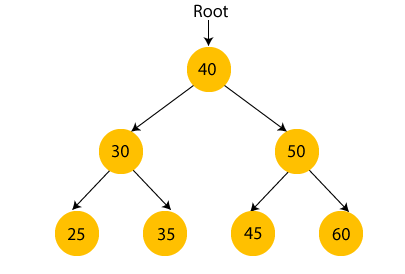
\includegraphics[scale=0.6]{Images/bst.png}
                \onslide<2>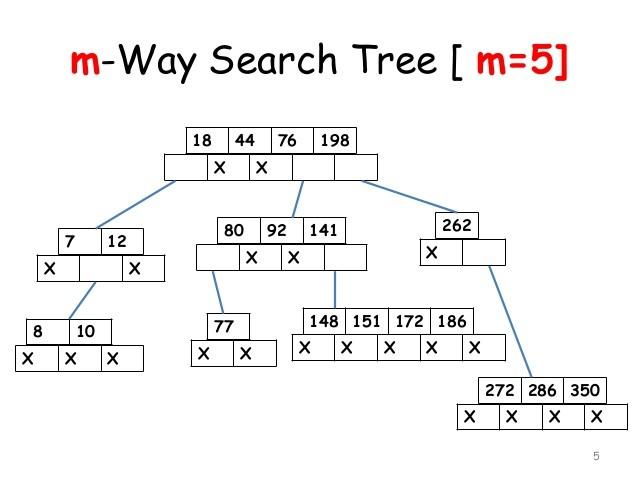
\includegraphics[scale=0.38]{Images/mwaytree.jpg}
                \onslide<3>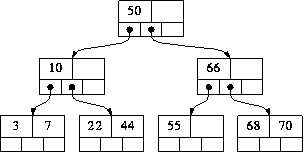
\includegraphics[scale=0.7]{Images/btree.png}
                \onslide<4>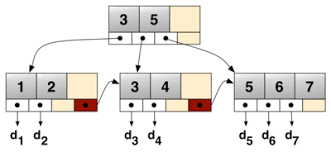
\includegraphics[scale=0.7]{Images/b+tree1.png}
            \end{overprint}
        \end{tabular}
    \end{table}
\end{frame}
\section{Properties of B+ Tree}
\begin{frame}{Structure of Nodes}
`   \begin{figure}
        \includegraphics[scale = 0.4]{Images/InternalNodeStructure.jpg}
        \caption{Internal Node Structure}
    \end{figure}
    \begin{figure}
        \includegraphics[scale = 0.35]{Images/Leaf3.png}
        \caption{Leaf Node Structure}
    \end{figure} 
\end{frame}

\begin{frame}{Node Bounds} 
    \begin{table}[h]
        \centering
        \begin{tabular}{| c | c | c | c | c |}
            \hline
              \textbf{Node} & \textbf{Min} & \textbf{Max} & \textbf{Min} & \textbf{Max}\\
              \textbf{Type} &\textbf{\#Keys}&\textbf{\#Keys}& \textbf{\#Child}&\textbf{\#Child}\\
              \hline
              
              Root & \multirow{2}{*}{1}&\multirow{2}{*}{$M-1$}&\multirow{2}{*}{2\cite{navathe2010fundamentals}}&\multirow{2}{*}{M}\\
              Node & & & & \\
              \hline
               Internal& \multirow{2}{*}{$\lceil{\frac{M}{2}}\rceil - 1$ }&\multirow{2}{*}{$M-1$} &  \multirow{2}{*}{$\lceil{\frac{M}{2}}\rceil $ } & \multirow{2}{*}{M}\\
               Node& & & & \\
             \hline
             Leaf & \multirow{2}{*}{$\lceil{\frac{M}{2}}\rceil - 1 $ }&\multirow{2}{*}{$M-1$} & \multirow{2}{*}{0} & \multirow{2}{*}{0}\\
               Node& & & & \\
             \hline

        \end{tabular}
    \end{table}
           M = Order of B+ Tree
\end{frame}
\section{Operations on B+ Tree}
\begin{frame}{Operations on B+ Tree}
    \centering
    {\huge\alert{HOW} do We Operate on B+ Tree?}
\end{frame}

\begin{frame}{B+ Tree Insertion}
    \begin{table}[]
        \centering
        \alert{\textbf{\huge{Insertion}}}
    \end{table}
    
\end{frame}

\begin{frame}{B+ Tree Insertion}
    \begin{block}{How to insert}
        Since every element is inserted into the leaf node, go to the appropriate leaf node. Insert the key into the leaf node.
    \end{block}
    \onslide<1->{
    \begin{block}{Case I:}
        If the leaf is not full, insert the key into the leaf node in increasing order.
    \end{block} }
    \onslide<2->{
    \begin{block}{Case II:}
        \begin{enumerate}
            \item If the leaf is full, insert the key into the leaf node in increasing order and balance the tree in the following way.
            \item Break the node at $\frac{m}{2}$ th position.
            \item Add $\frac{m}{2}$ th key to the parent node as well.
            \item If the parent node is already full, follow steps 2 to 3.
        \end{enumerate}
    \end{block} }
\end{frame}

\begin{frame}{B+ Tree Insertion Animation : \alert{Insert 5}}
    \begin{table}[h]
        \centering
        \begin{figure}
       
            \centering
            
\includegraphics[scale=0.8]{Images/bi1.jpg}
        \end{figure}
         \alert{Order = 3}
    \end{table} 
\end{frame}
\begin{frame}{B+ Tree Insertion Animation : \alert{Insert 15}}
    \begin{table}[h]
        \centering
        \begin{figure}
       
            \centering
            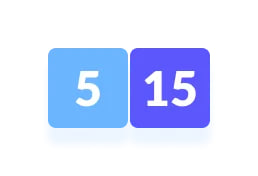
\includegraphics[scale=0.8]{Images/bi2.jpg}
        \end{figure}
    \end{table} 
\end{frame}
\begin{frame}{B+ Tree Insertion Animation : \alert{Insert 25}}
    \begin{table}[h]
        \centering
        \begin{overprint}
        \onslide<1>
        \begin{figure}
       
            \centering
            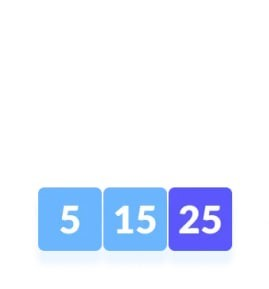
\includegraphics[scale=0.8]{Images/bi3_1_1.jpg}
        \end{figure}
        \onslide<2>\begin{figure}
            \centering
            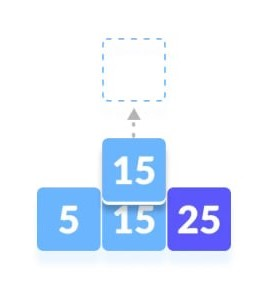
\includegraphics[scale=0.8]{Images/bi3_1_2.jpg}
        \end{figure}
        \onslide<3>\begin{figure}
            \centering
            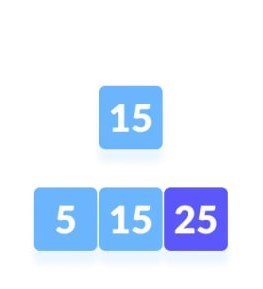
\includegraphics[scale=0.8]{Images/bi3_2_1.jpg}
        \end{figure}
        \onslide<4>\begin{figure}
            \centering
            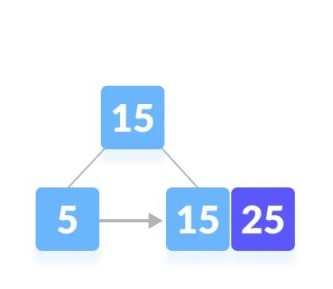
\includegraphics[scale=0.8]{Images/bi3_2_2.jpg}
        \end{figure}
        \end{overprint}
    \end{table} 
\end{frame}

\begin{frame}{B+ Tree Insertion Animation : \alert{Insert 35}}
    \begin{table}[h]
        \centering
        \begin{overprint}
        \onslide<1>
        \begin{figure}
       
            \centering
            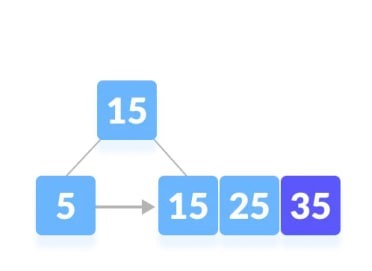
\includegraphics[scale=0.8]{Images/bi4_1_1.jpg}
        \end{figure}
        \onslide<2>\begin{figure}
            \centering
            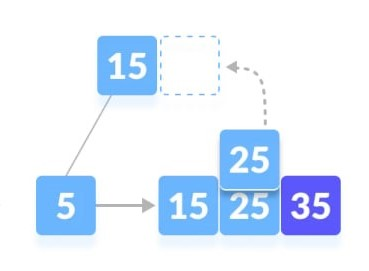
\includegraphics[scale=0.8]{Images/bi4_1_2.jpg}
        \end{figure}
        \onslide<3>\begin{figure}
            \centering
            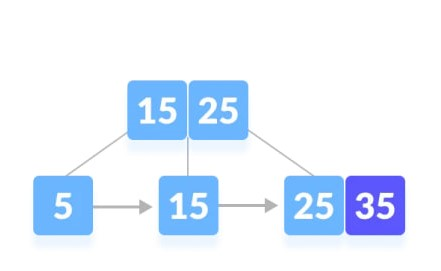
\includegraphics[scale=0.8]{Images/bi4_2.jpg}
        \end{figure}
        \end{overprint}
    \end{table} 
\end{frame}

\begin{frame}{B+ Tree Insertion Animation : \alert{Insert 45}}
    \begin{table}[h]
        \centering
        \begin{overprint}
        \onslide<1>
        \begin{figure}
       
            \centering
            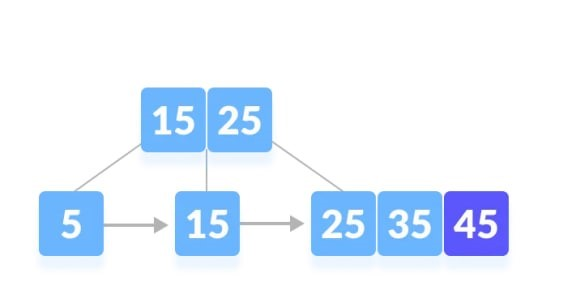
\includegraphics[scale=0.8]{Images/bi5_1_1.jpg}
        \end{figure}
        \onslide<2>\begin{figure}
            \centering
            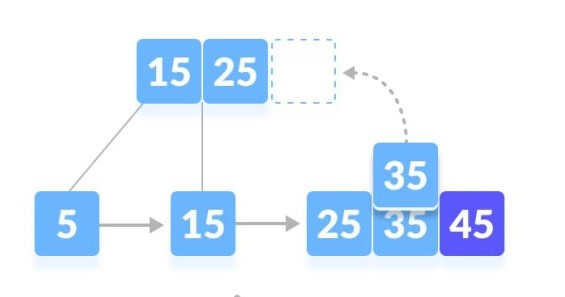
\includegraphics[scale=0.8]{Images/bi5_1_2.jpg}
        \end{figure}
        \onslide<3>\begin{figure}
            \centering
            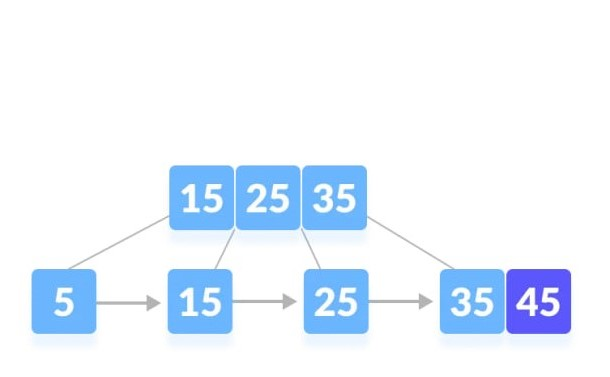
\includegraphics[scale=0.8]{Images/bi5_2_1.jpg}
        \end{figure}
        \onslide<4>\begin{figure}
            \centering
            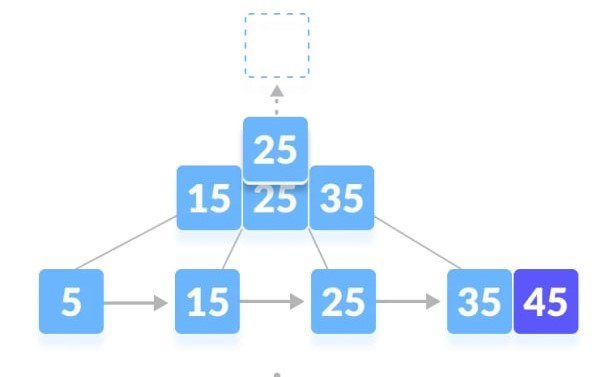
\includegraphics[scale=0.8]{Images/bi5_2_2.jpg}
        \end{figure}
        \onslide<5>\begin{figure}
            \centering
            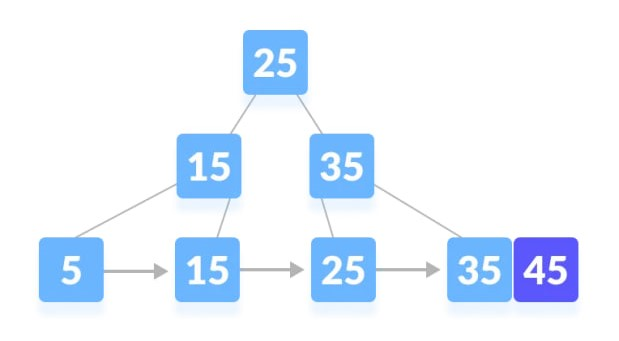
\includegraphics[scale=0.8]{Images/bi5_3.jpg}
        \end{figure}
        \end{overprint}
    \end{table} 
\end{frame}

\begin{frame}{B+ Tree Deletion}
    \begin{table}[]
        \centering
        \alert{\textbf{\huge{Deletion}}}
    \end{table}
\end{frame}

\begin{frame}{B+ Tree Deletion}
    Before going through the steps below, one must know these facts about a B+ tree of degree m. A node can have -
    \begin{enumerate}
        \item a maximum of m children. (i.e. 3)
        \item a maximum of m - 1 keys. (i.e. 2)
        \item a minimum of $\lceil m/2 \rceil$ children. (i.e. 2)
        \item a minimum of $\lceil m/2 \rceil - 1$ keys (except root node). (ie 1) \end{enumerate} \vspace{20pt}* In our example m = 3
\end{frame}

\begin{frame}{B+ Tree Deletion Animation}
    \begin{table}[h]
        \centering
        \begin{overprint}
        \onslide<1>
        \begin{block}{Case 1}
              The key to be deleted is present only in the leaf node and not in the internal nodes. For instance 5.
        \end{block}
            
        \begin{figure}
            \centering
             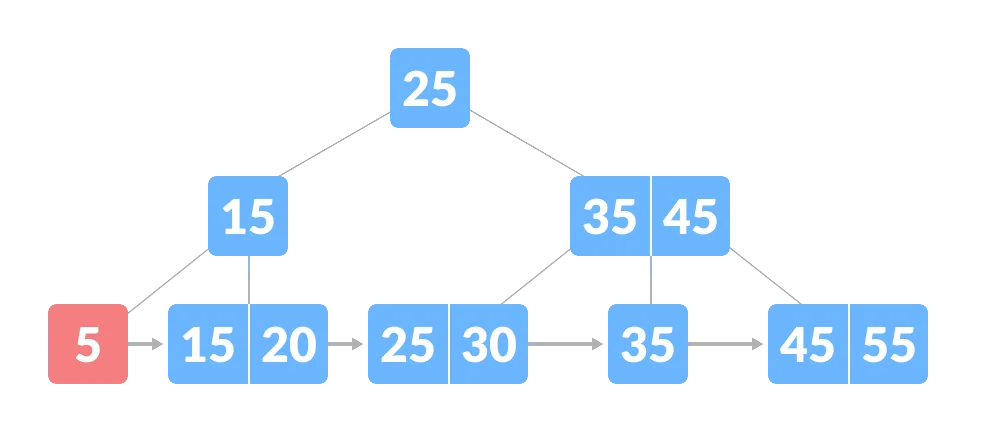
\includegraphics[scale=0.4]{Images/deletion-1.1.png}
        \end{figure}
        \onslide<2>\begin{figure}
            \centering
             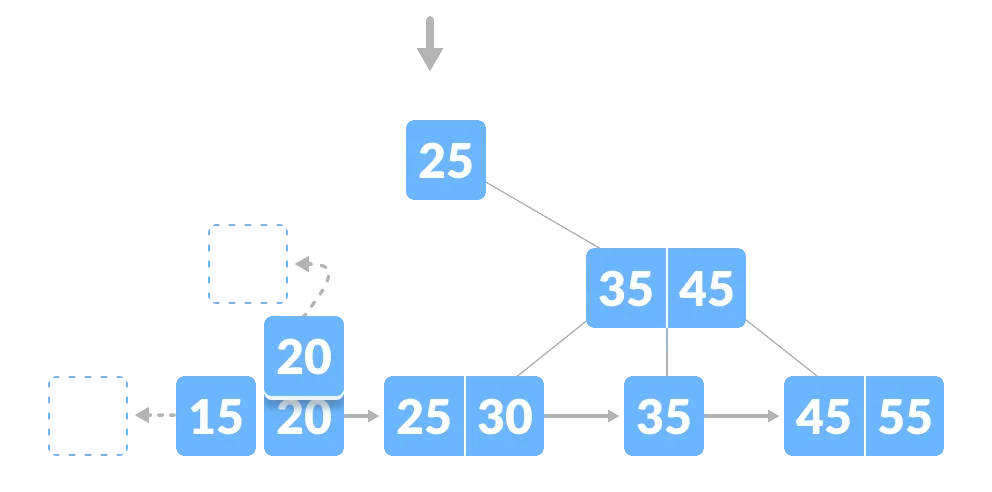
\includegraphics[scale=0.4]{Images/deletion-1.2.png}
        \end{figure}
        \onslide<3>\begin{figure}
            \centering
             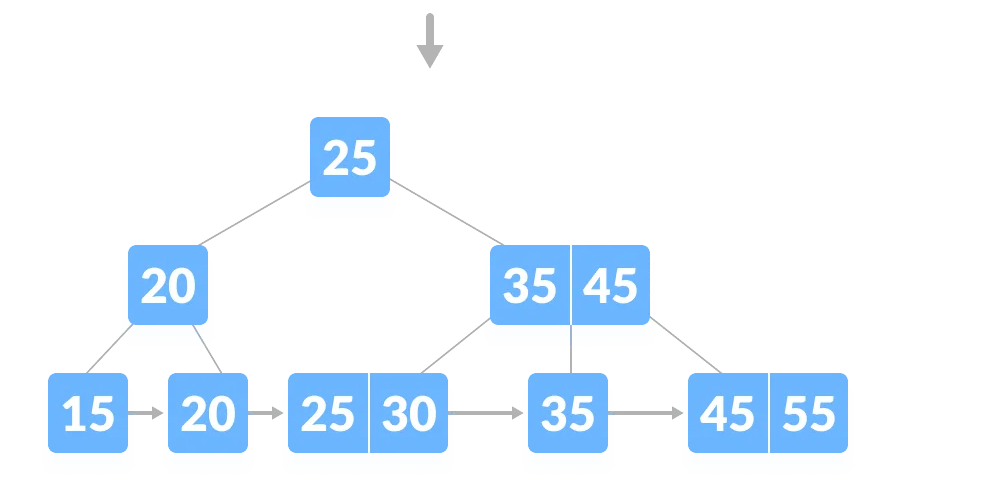
\includegraphics[scale=0.4]{Images/deletion-1.3.png}
        \end{figure}
        \onslide<4>\begin{block}{Case 2}
              The key to be deleted is present in the internal nodes as well. For example, 45.
        \end{block}
        \begin{figure}
            \centering
              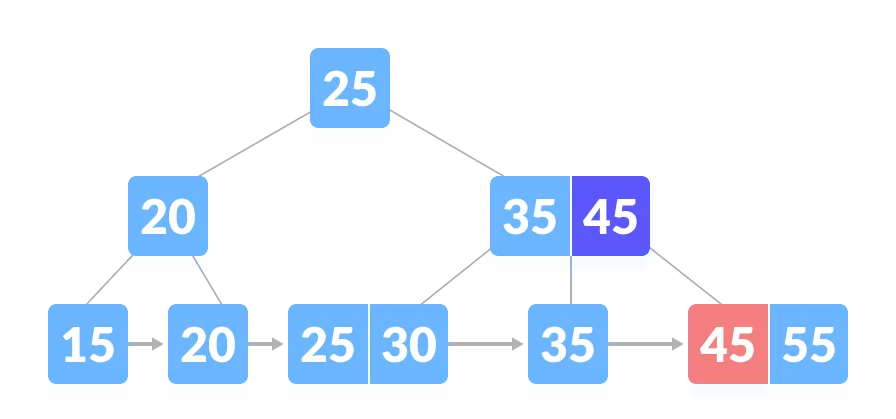
\includegraphics[scale=0.4]{Images/deletion-3.1.png}
        \end{figure}
        \onslide<5>\begin{figure}
             \centering
             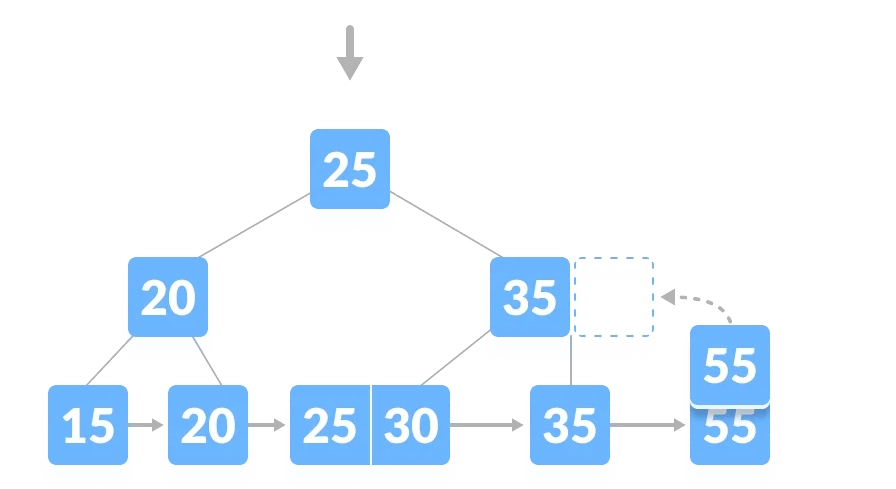
\includegraphics[scale=0.4]{Images/deletion-3.2.png}
        \end{figure}
        \onslide<6>\begin{figure}
             \centering
             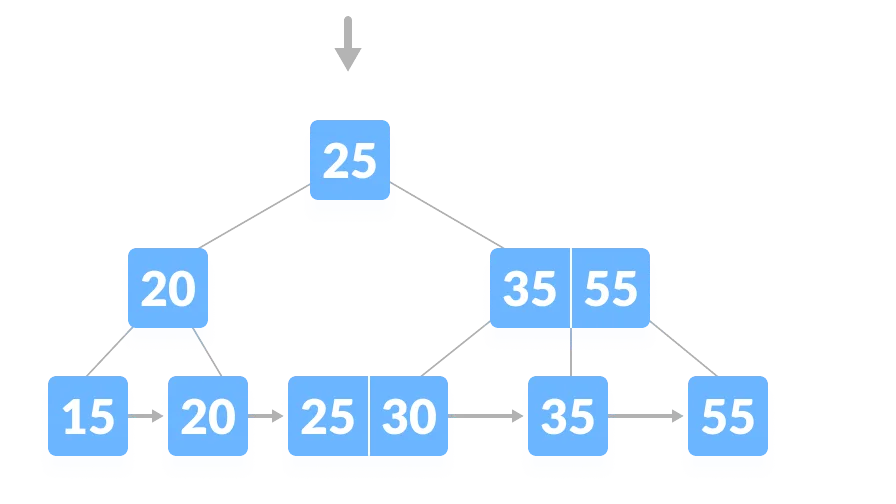
\includegraphics[scale=0.4]{Images/deletion-3.3.png}
        \end{figure}
        \onslide<7>\begin{figure}
            \centering
            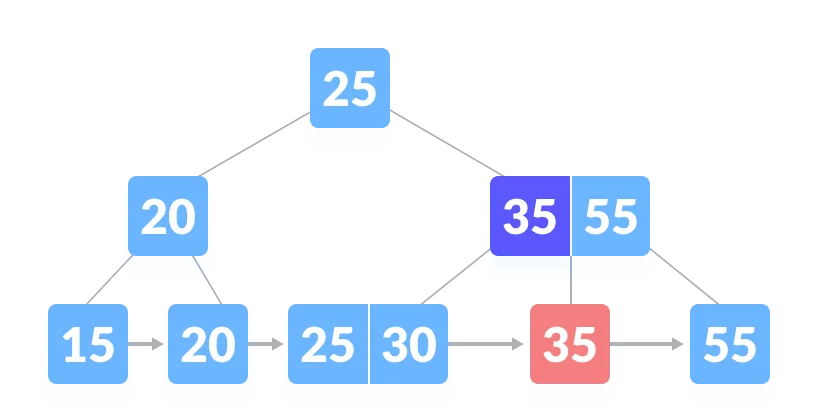
\includegraphics[scale=0.4]{Images/deletion-4.1.png}
        \end{figure}
        \onslide<8>\begin{figure}
            \centering
             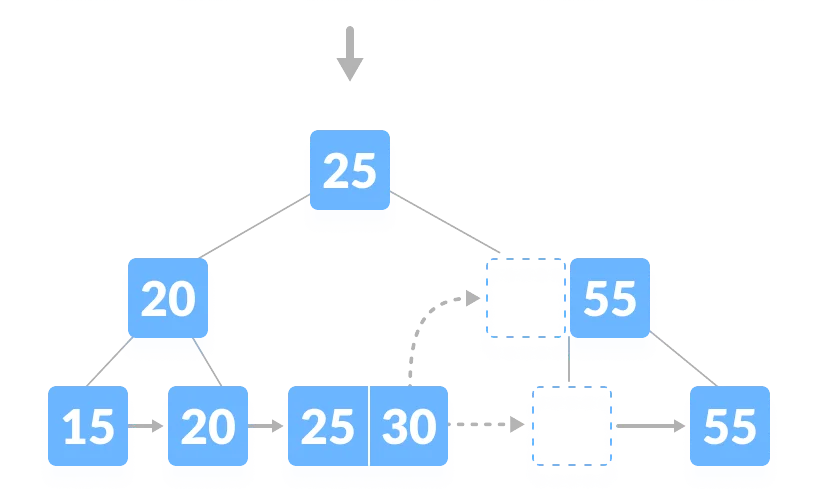
\includegraphics[scale=0.4]{Images/deletion-4.2.png}
        \end{figure}
        \onslide<9>\begin{figure}
             \centering
             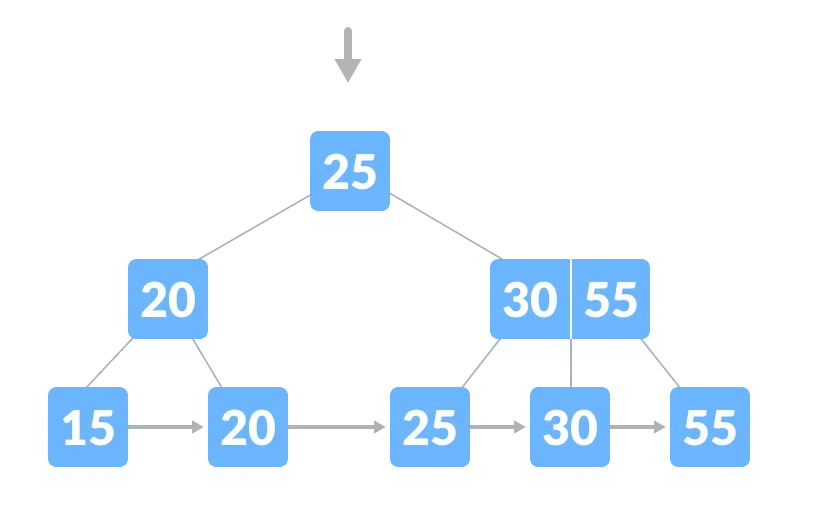
\includegraphics[scale=0.4]{Images/deletion-4.3.png}
        \end{figure}
        \onslide<10>\begin{figure}
            \centering
              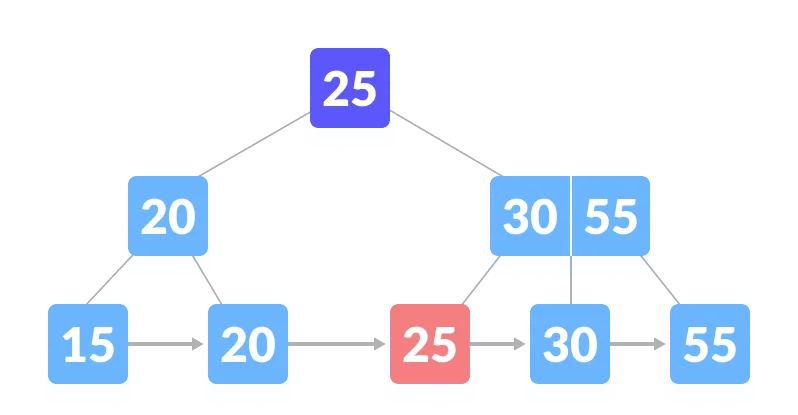
\includegraphics[scale=0.4]{Images/deletion-5.1.png}
        \end{figure}
        \onslide<11>\begin{figure}
             \centering
             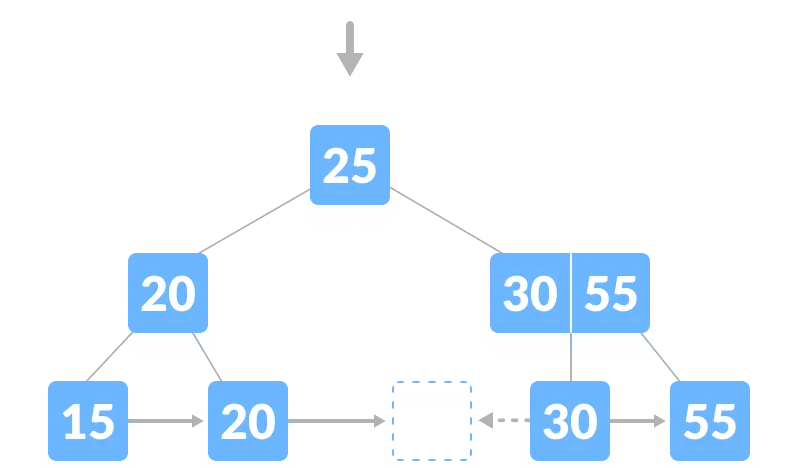
\includegraphics[scale=0.4]{Images/deletion-5.2.png}
        \end{figure}
        \onslide<12>\begin{figure}
             \centering
             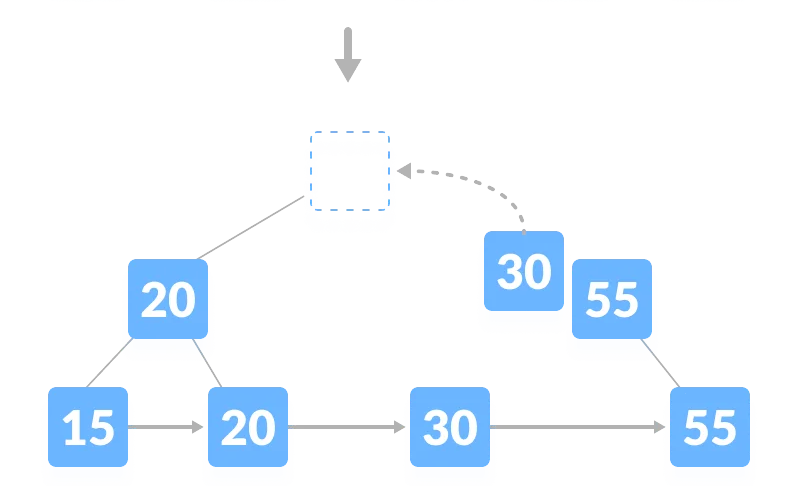
\includegraphics[scale=0.4]{Images/deletion-5.3.png}
        \end{figure}
        \onslide<13>\begin{figure}
            \centering
             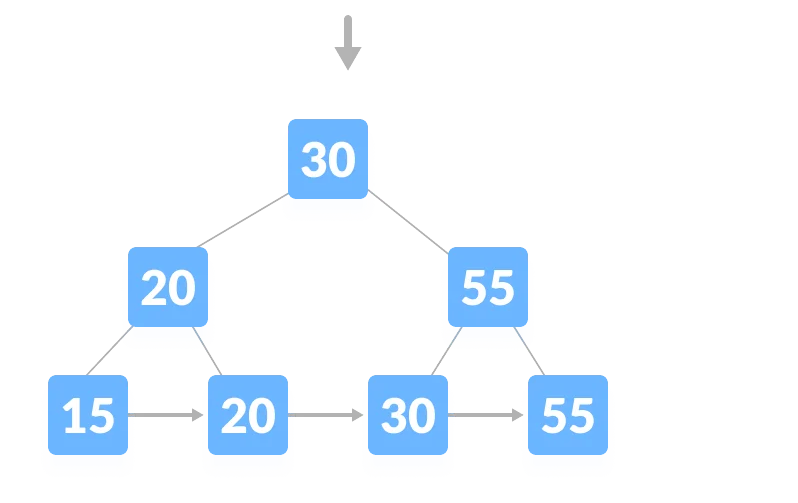
\includegraphics[scale=0.4]{Images/deletion-5.4.png}
        \end{figure}
        \onslide<14>\begin{block}{Case 3}
            The height of the tree gets shrinked. For example deletion of 55.
        \end{block}
        \begin{figure}
             \centering
             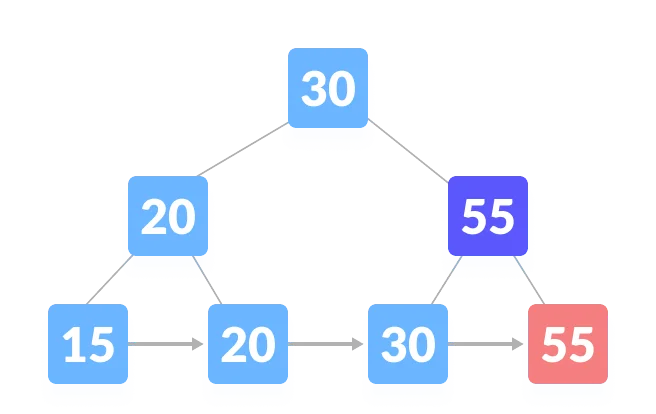
\includegraphics[scale=0.4]{Images/deletion-6.1.png}
        \end{figure}
        \onslide<15>\begin{figure}
            \centering
              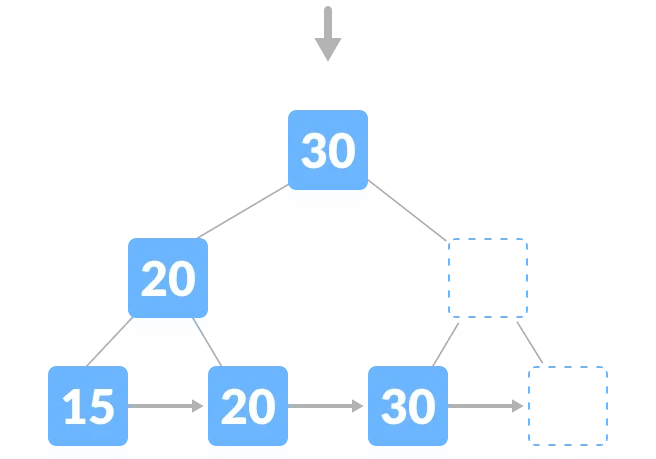
\includegraphics[scale=0.4]{Images/deletion-6.2.png}
        \end{figure}
        \onslide<16>\begin{figure}
             \centering
             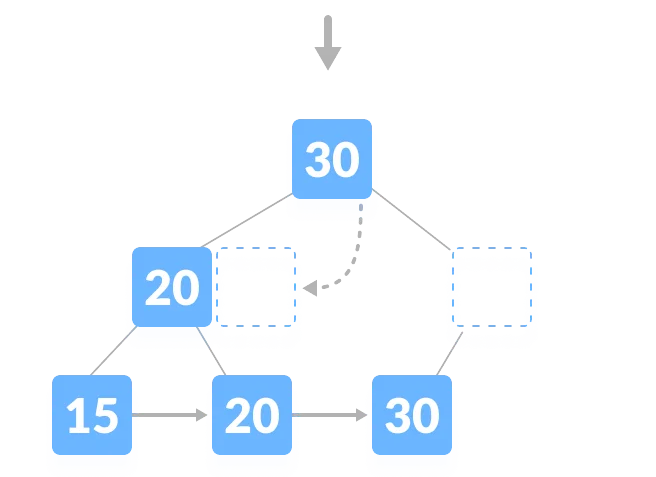
\includegraphics[scale=0.4]{Images/deletion-6.3.png}
        \end{figure}
        \onslide<17>\begin{figure}
             \centering
             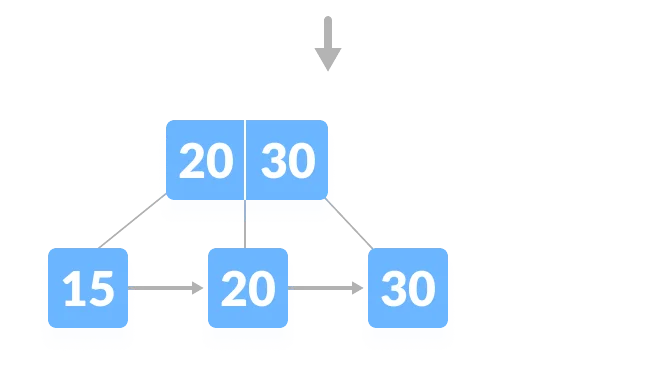
\includegraphics[scale=0.4]{Images/deletion-6.4.png}
        \end{figure}
        \end{overprint}
    \end{table} 
\end{frame}

\begin{frame}{Importance of B+ Tree}
    \centering
    {\huge\alert{WHY} do We Actually Need B+ Tree?}
\end{frame}

\begin{frame}{Time Analysis}

    \begin{overlayarea}{\textwidth}{\textheight}
    \vspace{50pt} % adjust vertical spacing
    \begin{table}
        \centering
        \small % adjust font size
        \setlength{\tabcolsep}{10pt} % adjust column spacing
        \renewcommand{\arraystretch}{1.5} % adjust row spacing
        \begin{tabular}{|c|c|}
            \hline
            \textbf{B+ Tree Operation} & \textbf{Time Complexity}  \\
            \hline
            \onslide<1->{Insertion} & \onslide<1->{$O(\log_m n)$}\\
            \hline
            \onslide<2->{Deletion} & \onslide<2->{$O(\log_m n)$}\\
            \hline
            \onslide<3->{Search} & \onslide<3->{$O(\log_m n)$}\\
            \hline
        \end{tabular}
    \end{table}
    \vspace{10pt} % adjust vertical spacing
    $m =$ Order of B+ Tree\\
    $n =$ Number of elements in B+ Tree
    \end{overlayarea}
\end{frame}

\section{Advantages of B+ Trees}

\begin{frame}{B+ Tree}
    \centering
    {\huge Advantages of B+ Trees}
\end{frame}

\begin{frame}
    \frametitle{Advantages of B+ Trees}
    \begin{block}{Ordered Structure for Sequential Access}
    B+ trees maintain data in sorted order, facilitating efficient sequential access to keys. \cite{garcia2000database}.
    \end{block}
\end{frame}

\begin{frame}
    \frametitle{Advantages of B+ Trees (Cont'd)}
    \begin{block}{Concurrency Control and Performance} 
        B+ trees supports locking and MVCC to ensure consistency and isolation among concurrent transactions \cite{agrawal1987concurrency}.
    \end{block}
\end{frame}

\begin{frame}
    \frametitle{Advantages of B+ Trees (Cont'd)}
    \begin{block}{Optimal Disk Access and Cache Efficiency}
        B+ trees utilize node-based structures and node sizes that align well with the block size of storage devices, minimizing disk access and maximizing cache hits \cite{oneil1992modern}.
    \end{block}
\end{frame}


\section{Real Life Application of B+ Tree}

\begin{frame}{Real Life Application of B+ Tree}
    \centering
    {\huge\alert{WHERE} do We Use B+ Trees in Real Life?}
\end{frame}

\begin{frame}{B+ Tree}
    \centering
    {\huge Real Life Application of B+ Tree}
\end{frame}

\begin{frame}{Real Life Application of B+ Tree}
    \begin{block}{Database Indexing}
        B+ trees enable effective retrieval of data based on indexed characteristics, resulting in faster query execution times.
    \end{block}
\end{frame}

\begin{frame}{Real Life Application of B+ Tree}
    \begin{block}{Web Browsers}
        B+ trees are employed in web browsers for managing bookmarks and history data.
    \end{block}
\end{frame}

\begin{frame}{Real Life Application of B+ Tree}
    \begin{block}{Geo-spatial Databases}
        B+ trees are well-suited for indexing geo-spatial data such as coordinates, shapes, and spatial relationships.
    \end{block}
\end{frame}

\begin{frame}
    \begin{figure}
        \centering
        
\includegraphics[scale=0.6]{Images/endOfSlide.jpg}
    \end{figure}
\end{frame}

\begin{frame}[allowframebreaks]{References}
    \bibliographystyle{plain}
    \bibliography{References}
\end{frame}

\end{document}
